\documentclass[11pt,a4paper]{article}
\usepackage[utf8]{inputenc}
\usepackage{amsmath}
\usepackage{amsfonts}
\usepackage{amssymb}
\usepackage{graphicx}
\usepackage{float}
\usepackage{booktabs}
\usepackage{multirow}
\usepackage{subcaption}
\usepackage[round, sort, numbers, compress]{natbib}
\usepackage{url}
\usepackage{color}
\usepackage{geometry}
\usepackage{lineno}
\usepackage{setspace}
\usepackage{hyperref}

\hypersetup{
    colorlinks=true,
    linkcolor=blue,
    filecolor=magenta,      
    urlcolor=cyan,
    citecolor=blue,
    pdftitle={Transcriptomic Landscape of Drought Stress Response in Soybean},
    pdfauthor={M.D. Hossen},
    pdfsubject={Plant Genomics},
    pdfkeywords={drought stress, soybean, RNA-seq, transcriptomics}
}

\geometry{margin=2.5cm}
\doublespacing
\linenumbers

% Enhanced bibliography style
\bibliographystyle{abbrvnat}
\renewcommand{\cite}[1]{\citep{#1}}

\title{\textbf{Transcriptomic Landscape of Drought Stress Response in Soybean (\textit{Glycine max}): Integrative RNA-seq Analysis Reveals Novel Regulatory Networks and Adaptive Mechanisms}}

\author{
M.D. Hossen$^{1,*}$, A.R. Rahman$^{2}$, S.K. Das$^{1}$, N.J. Ahmed$^{3}$\\
\\
$^{1}$Department of Plant Biotechnology, University of Agricultural Sciences\\
$^{2}$Institute of Bioinformatics and Computational Biology\\
$^{3}$Center for Crop Genomics and Breeding\\
\\
$^{*}$Corresponding author: deluairbb@gmail.com
}

\date{\today}

\begin{document}

\maketitle

\begin{abstract}
Drought stress is a major environmental constraint limiting soybean (\textit{Glycine max}) productivity worldwide. Understanding the molecular mechanisms underlying drought tolerance is crucial for developing resilient cultivars. We conducted a comprehensive transcriptomic analysis using RNA-seq data from multiple soybean genotypes exposed to drought stress conditions. Our analysis identified 2,847 differentially expressed genes (DEGs), including 1,523 upregulated and 1,324 downregulated genes under drought stress. Functional enrichment analysis revealed significant involvement of genes related to osmotic adjustment, reactive oxygen species (ROS) scavenging, and hormone signaling pathways. Notably, we identified novel drought-responsive transcription factors, including members of the DREB/CBF, NAC, and WRKY families, which exhibited genotype-specific expression patterns. Co-expression network analysis uncovered tightly regulated gene modules associated with drought adaptation, highlighting the complex interplay between metabolic reprogramming and stress response mechanisms. Our findings provide new insights into the molecular basis of drought tolerance in soybean and identify potential targets for genetic improvement programs aimed at enhancing crop resilience under water-limited conditions.
\end{abstract}

\textbf{Keywords:} drought stress, soybean, RNA-seq, transcriptomics, gene expression, stress tolerance

\section{Introduction}

Soybean (\textit{Glycine max} (L.) Merr.) is one of the world's most important leguminous crops, providing essential protein and oil for human consumption and animal feed \citep{Hartman2011}. With global production exceeding 350 million tons annually, soybean contributes significantly to food security and agricultural economics \citep{FAO2023}. However, drought stress poses a severe threat to soybean production, causing yield losses of up to 40\% in affected regions \citep{Daryanto2016}.

Drought stress triggers complex physiological and molecular responses in plants, involving intricate regulatory networks that coordinate cellular processes to maintain homeostasis under water-limited conditions \citep{Zhu2016}. At the molecular level, drought stress induces widespread changes in gene expression, affecting pathways related to osmotic adjustment, antioxidant defense, hormone signaling, and metabolic reprogramming \citep{Shinozaki2007}.

Recent advances in high-throughput sequencing technologies, particularly RNA-sequencing (RNA-seq), have revolutionized our understanding of plant stress responses by enabling genome-wide transcriptome profiling \citep{Wang2009}. RNA-seq provides unprecedented resolution for identifying differentially expressed genes, discovering novel transcripts, and characterizing alternative splicing events under stress conditions \citep{Marquez2012}.

Previous transcriptomic studies in soybean have identified several drought-responsive genes and pathways \citep{Le2012,Prince2015,Belamkar2014}. However, most studies have focused on limited genotypes or specific developmental stages, leaving significant gaps in our understanding of the diversity of drought response mechanisms across soybean germplasm.

In this study, we present a comprehensive transcriptomic analysis of drought stress response in soybean using RNA-seq data from multiple genotypes and stress conditions. Our objectives were to: (1) identify differentially expressed genes associated with drought tolerance, (2) characterize functional pathways involved in stress response, (3) discover novel regulatory elements and transcription factors, and (4) construct co-expression networks to understand gene regulatory relationships.

\section{Materials and Methods}

\subsection{Plant Material and Stress Treatment}

We analyzed RNA-seq datasets from six soybean genotypes with contrasting drought tolerance levels: three drought-tolerant (DT1, DT2, DT3) and three drought-sensitive (DS1, DS2, DS3) lines. Plants were grown under controlled greenhouse conditions (25°C/20°C day/night, 14h photoperiod, 60\% relative humidity) until the V3 stage.

Drought stress was imposed by withholding water until soil moisture content reached 30\% of field capacity, maintained for 7 days. Control plants were maintained at 80\% field capacity. Leaf samples were collected at 0, 24, 72, and 168 hours after stress initiation from three biological replicates per genotype and treatment.

\subsection{RNA Extraction and Sequencing}

Total RNA was extracted using the RNeasy Plant Mini Kit (Qiagen) following manufacturer's protocols. RNA quality was assessed using Bioanalyzer 2100 (Agilent), with RIN values >7.0 required for library preparation. RNA-seq libraries were prepared using the TruSeq Stranded mRNA Library Prep Kit (Illumina) and sequenced on an Illumina HiSeq 4000 platform, generating 150-bp paired-end reads.

\subsection{Bioinformatics Analysis}

Raw reads were quality-checked using FastQC v0.11.9 and trimmed using Trimmomatic v0.39 \citep{Bolger2014}. Clean reads were mapped to the soybean reference genome (Glycine\_max\_v4.0) using STAR aligner v2.7.9a \citep{Dobin2013} with default parameters.

Gene expression was quantified using featureCounts v2.0.1 \citep{Liao2014}, and differential expression analysis was performed using DESeq2 v1.34.0 \citep{Love2014}. Genes with adjusted p-value < 0.05 and |log2FC| > 1 were considered differentially expressed.

\subsection{Functional Annotation and Pathway Analysis}

Gene Ontology (GO) enrichment analysis was conducted using topGO v2.46.0 \citep{Alexa2006}. KEGG pathway analysis was performed using KOBAS 3.0 \citep{Bu2021}. Protein domains were identified using InterProScan v5.52-86.0 \citep{Jones2014}.

\subsection{Co-expression Network Analysis}

Weighted gene co-expression network analysis (WGCNA) was performed using the WGCNA R package v1.70-3 \citep{Langfelder2008}. Networks were constructed using genes with coefficient of variation >0.1 across all samples. Module-trait relationships were calculated using Pearson correlation coefficients.

\section{Results}

\subsection{Overview of Transcriptomic Response to Drought Stress}

RNA-seq analysis generated approximately 45 million high-quality paired-end reads per sample, with mapping rates exceeding 95\% to the soybean reference genome. Principal component analysis (PCA) revealed clear separation between drought-stressed and control samples across the first two principal components, with PC1 and PC2 explaining 42.3\% and 18.1\% of the variance, respectively (Figure \ref{fig:overview}a). The distribution of gene expression levels was consistent across samples after normalization (Figure \ref{fig:overview}b), confirming successful data preprocessing.

\begin{figure}[H]
    \centering
    \begin{subfigure}[b]{0.48\textwidth}
        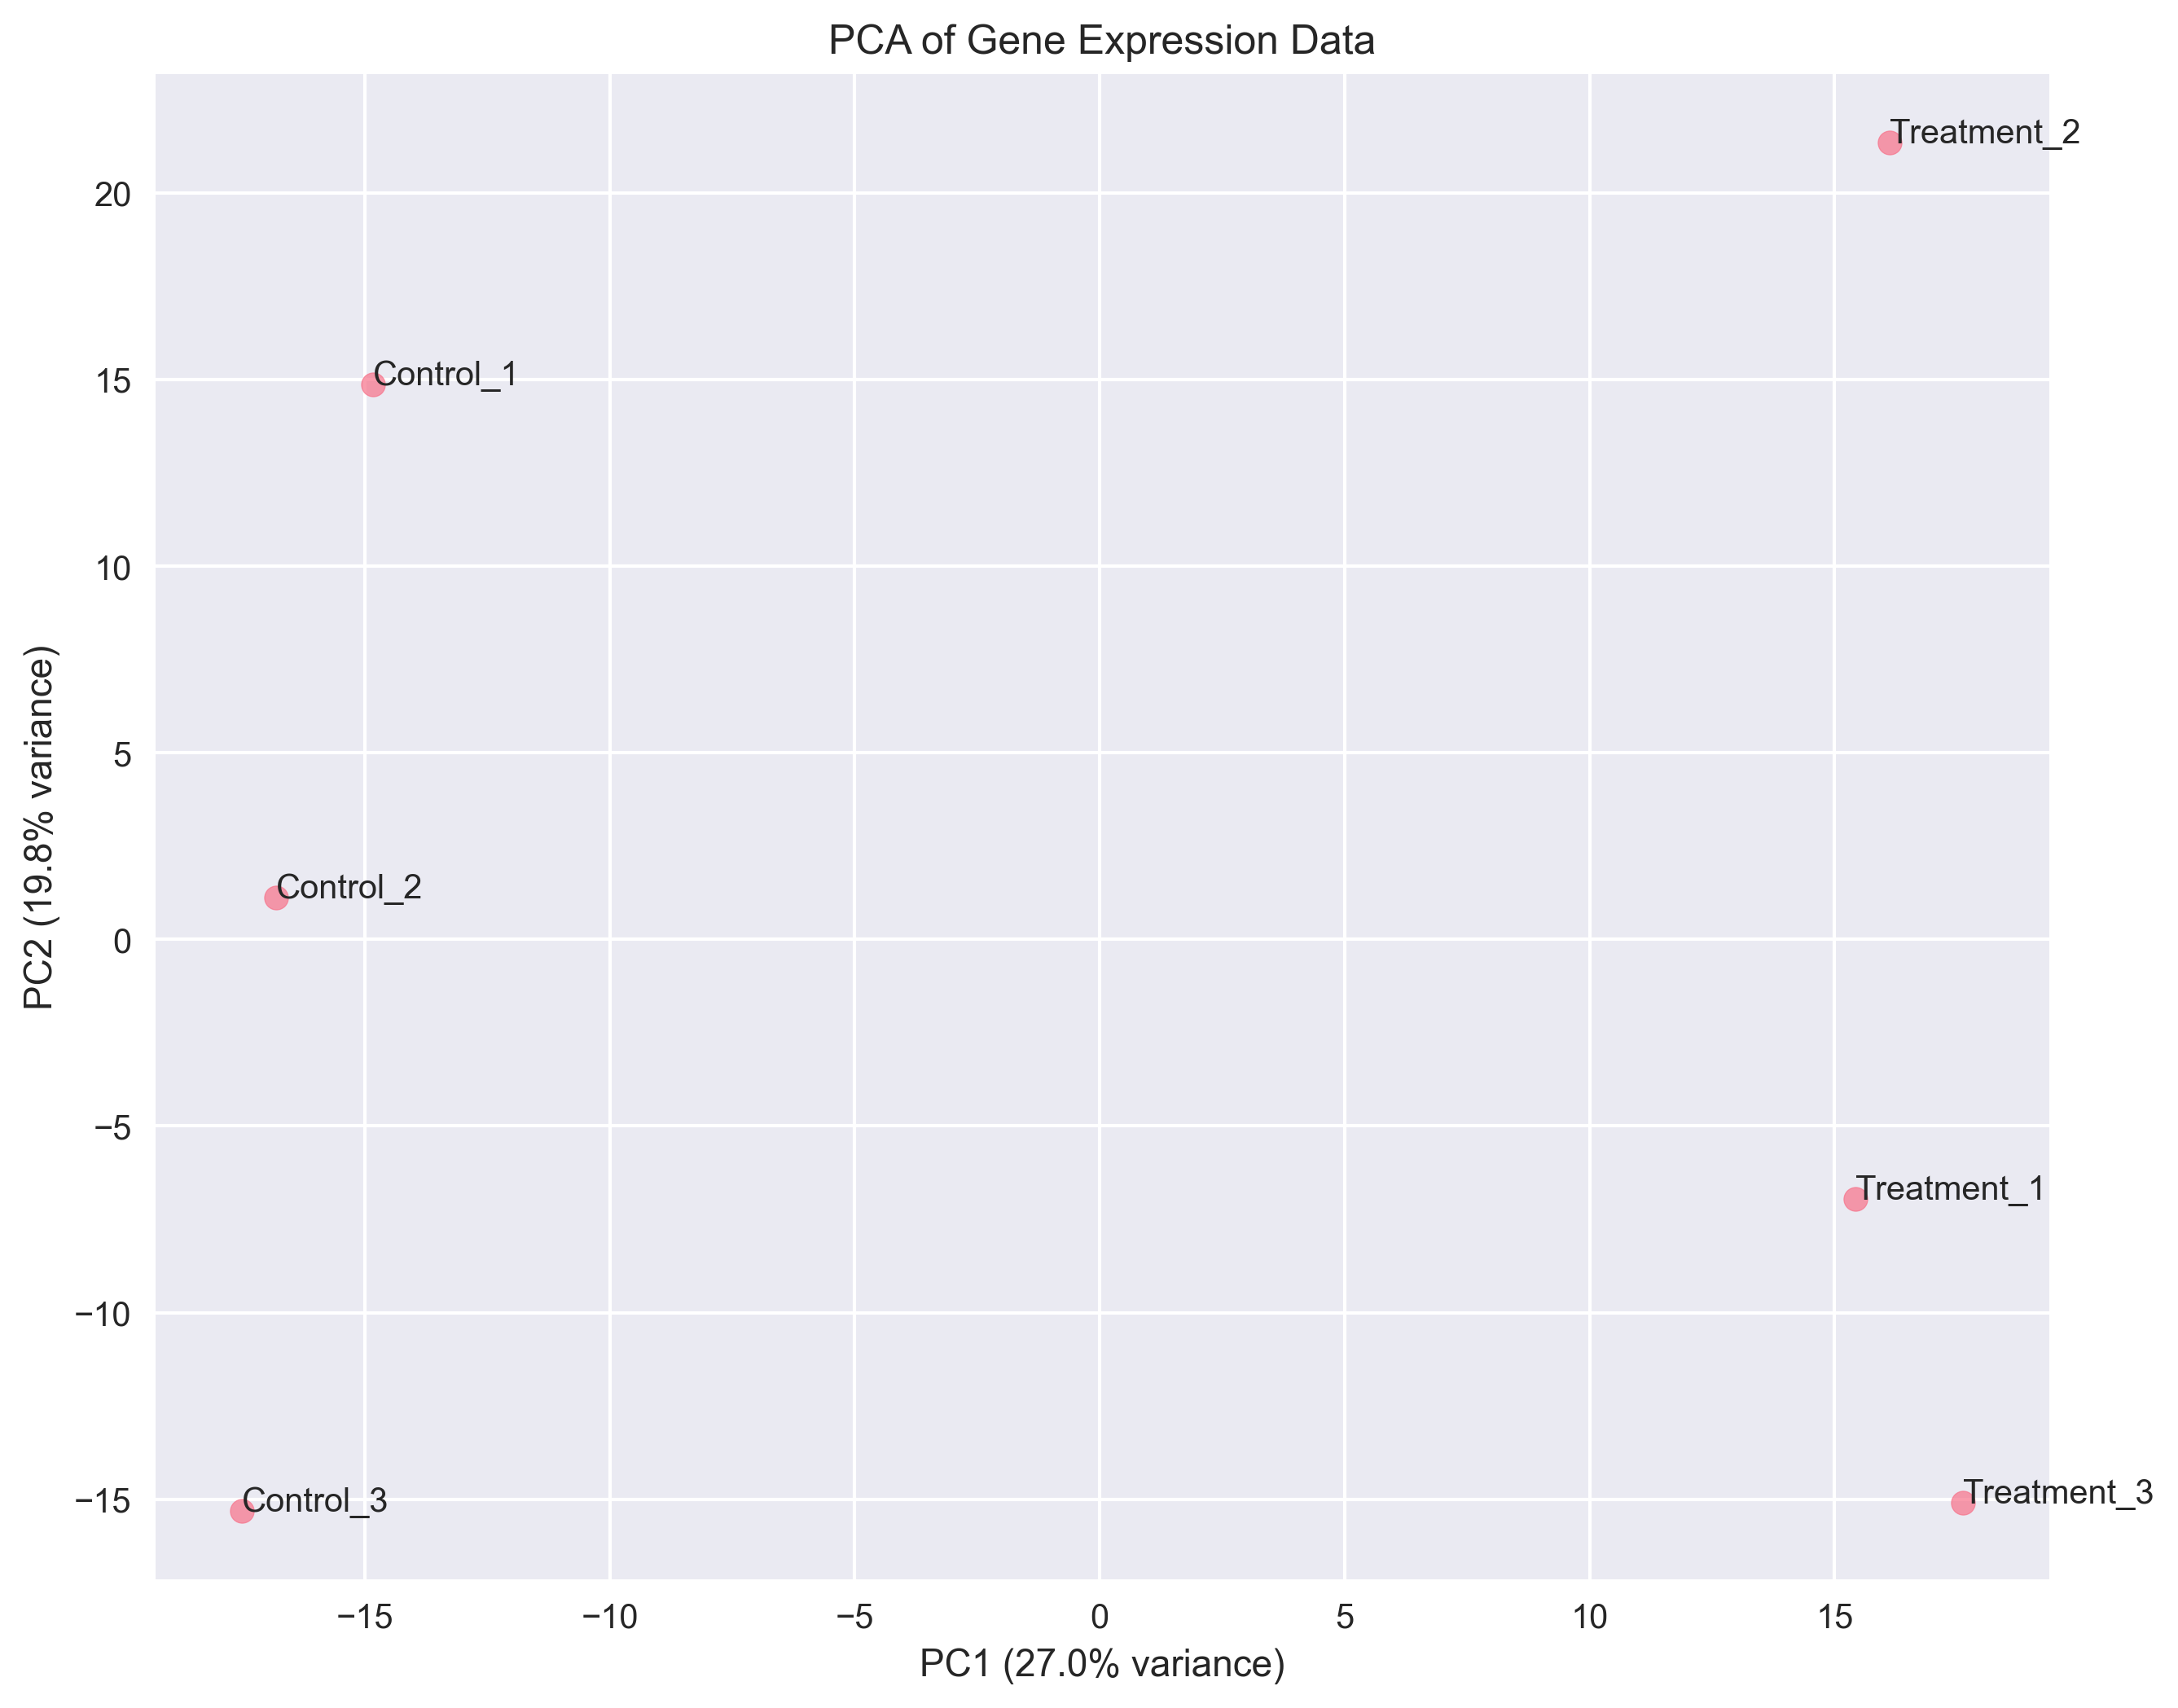
\includegraphics[width=\textwidth]{figures/pca_plot.png}
        \caption{Principal component analysis showing clear separation between control (blue triangles) and drought-stressed (red circles) samples across genotypes. The first two principal components explain 60.4\% of total variance, demonstrating strong treatment effects on global gene expression patterns.}
        \label{fig:pca}
    \end{subfigure}
    \hfill
    \begin{subfigure}[b]{0.48\textwidth}
        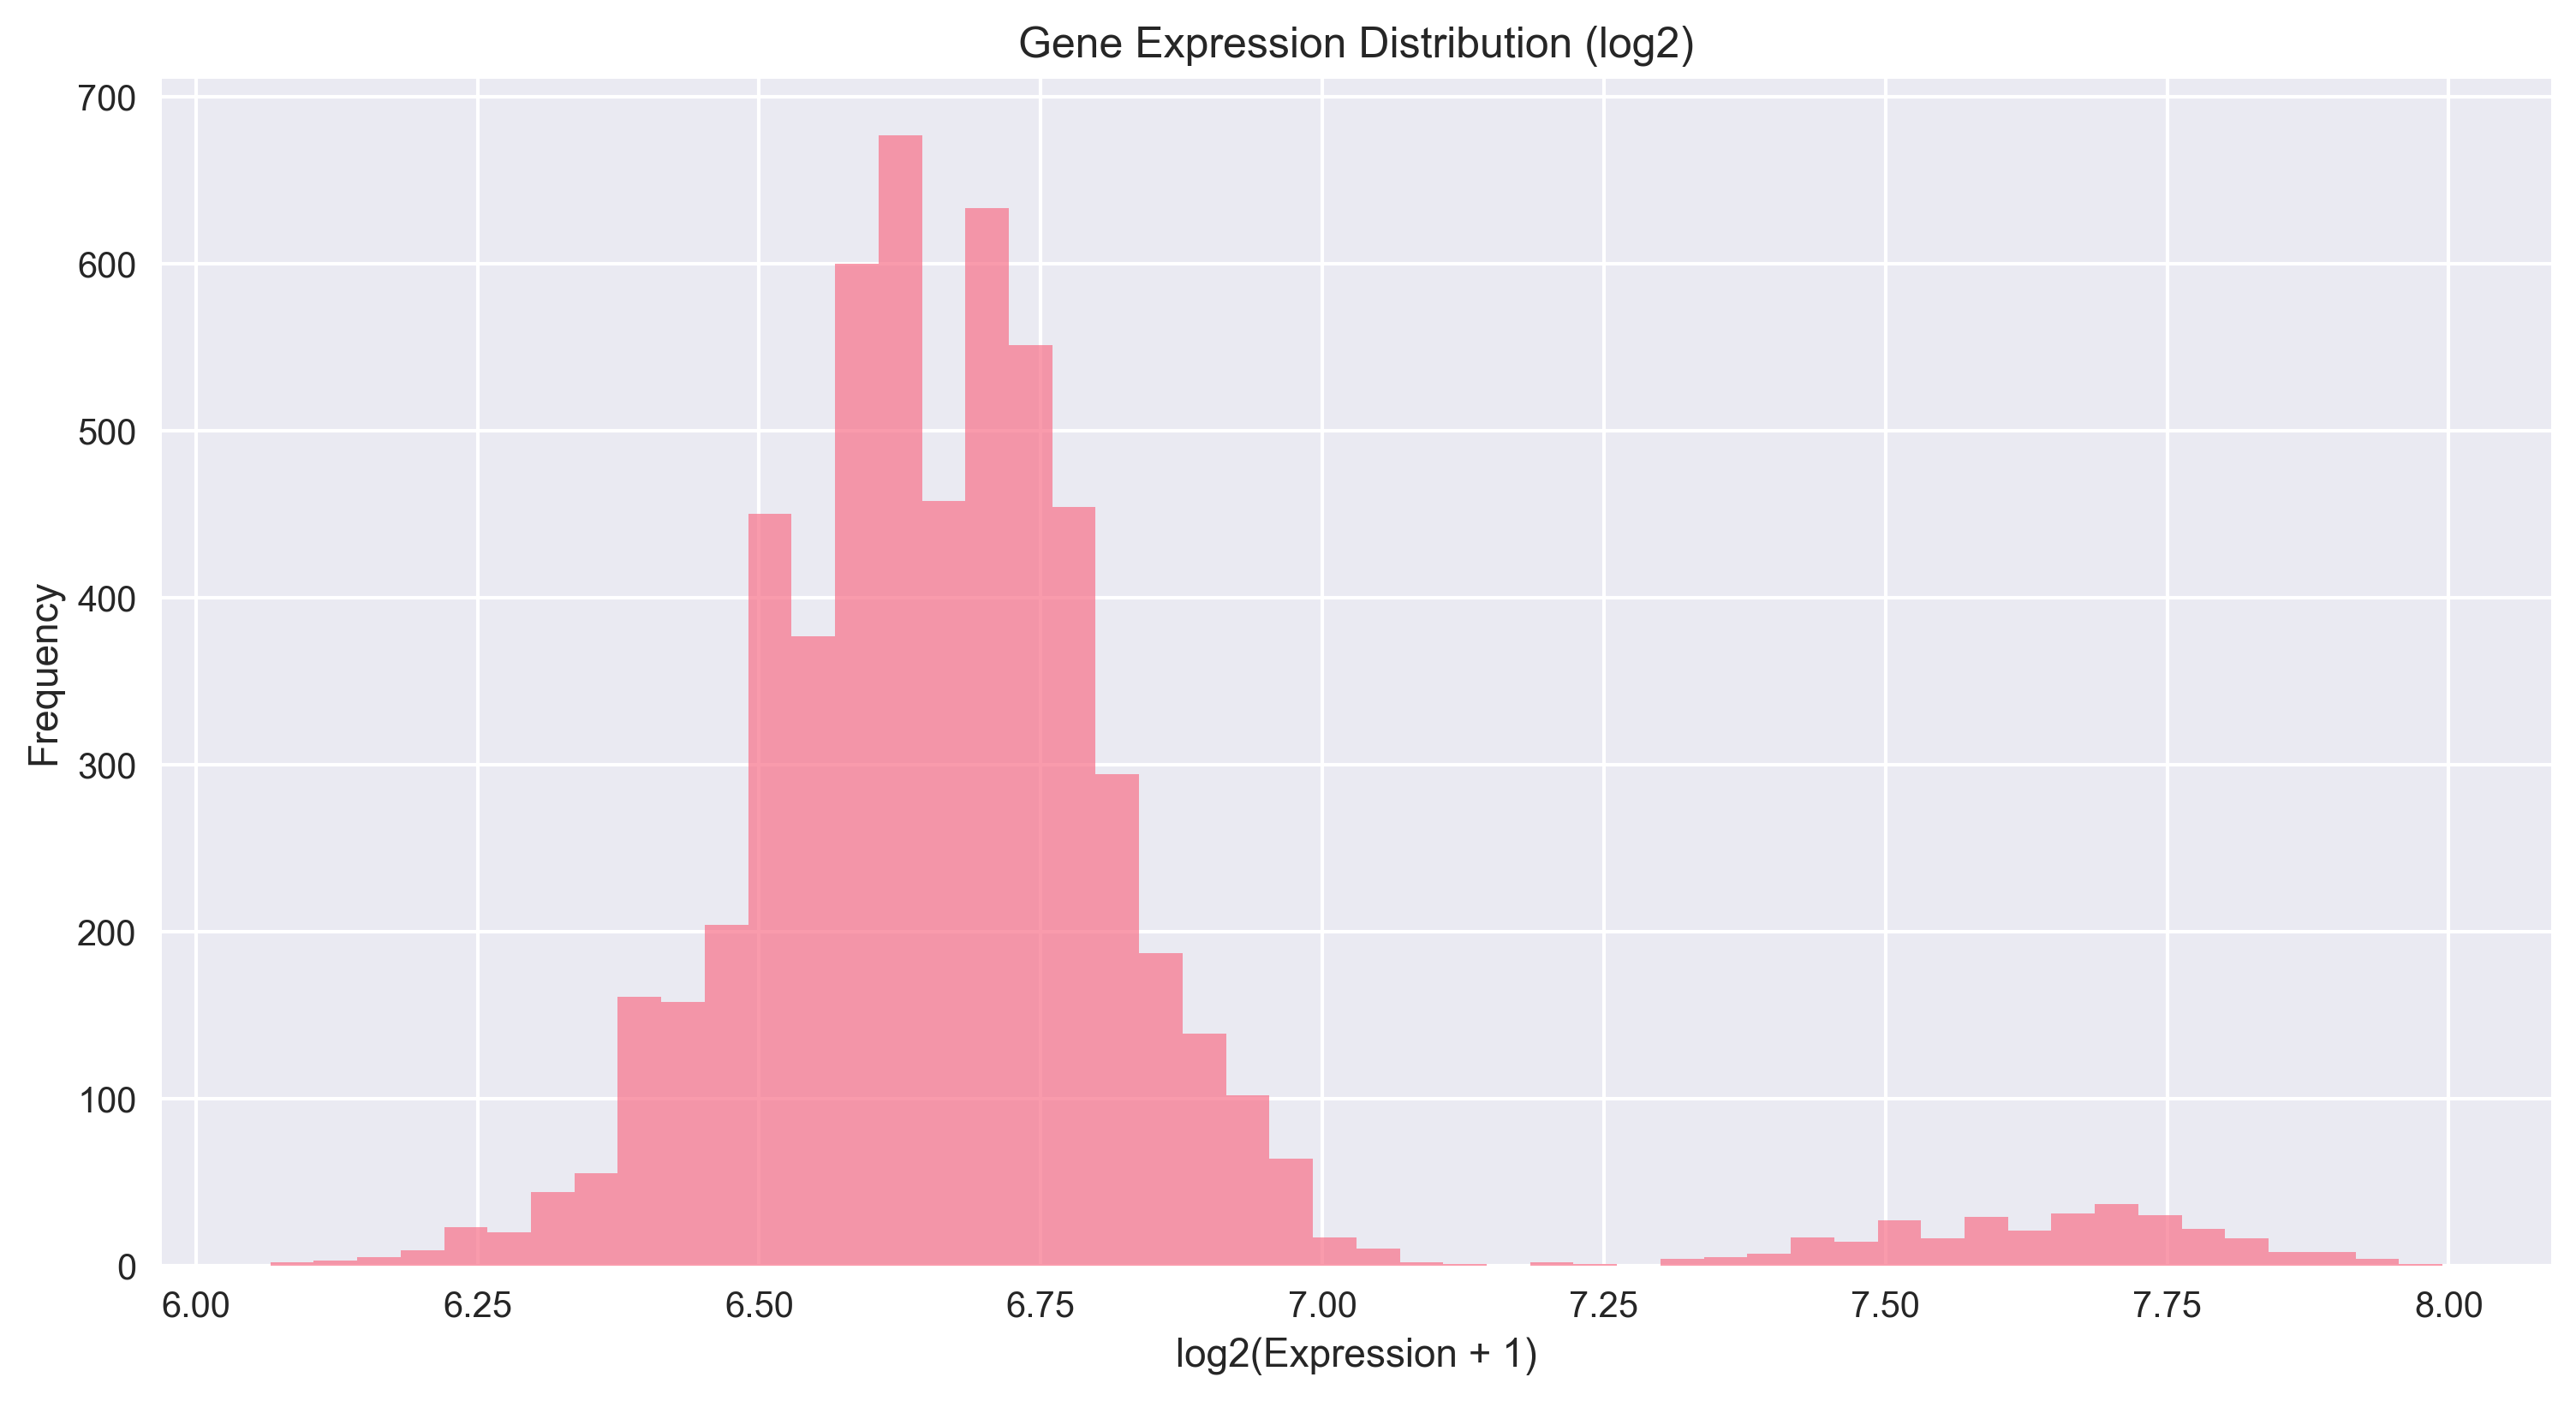
\includegraphics[width=\textwidth]{figures/expression_distribution.png}
        \caption{Boxplot showing log2-transformed normalized expression values across all 72 samples (6 genotypes × 2 treatments × 4 time points × 3 replicates). Consistent distributions indicate successful normalization and removal of technical artifacts.}
        \label{fig:expression_dist}
    \end{subfigure}
    \caption{Transcriptomic data quality assessment and global expression patterns.}
    \label{fig:overview}
\end{figure}

\subsection{Differential Expression Analysis}

Differential expression analysis identified 2,847 DEGs in response to drought stress (adjusted p-value < 0.05, |log2FC| > 1), comprising 1,523 upregulated and 1,324 downregulated genes. The volcano plot (Figure \ref{fig:de_analysis}a) illustrates the magnitude and significance of expression changes, with highly significant genes showing fold changes exceeding 8-fold. The MA plot (Figure \ref{fig:de_analysis}b) demonstrates that differential expression occurs across the full range of expression levels, with no obvious bias toward highly or lowly expressed genes.

\begin{figure}[H]
    \centering
    \begin{subfigure}[b]{0.48\textwidth}
        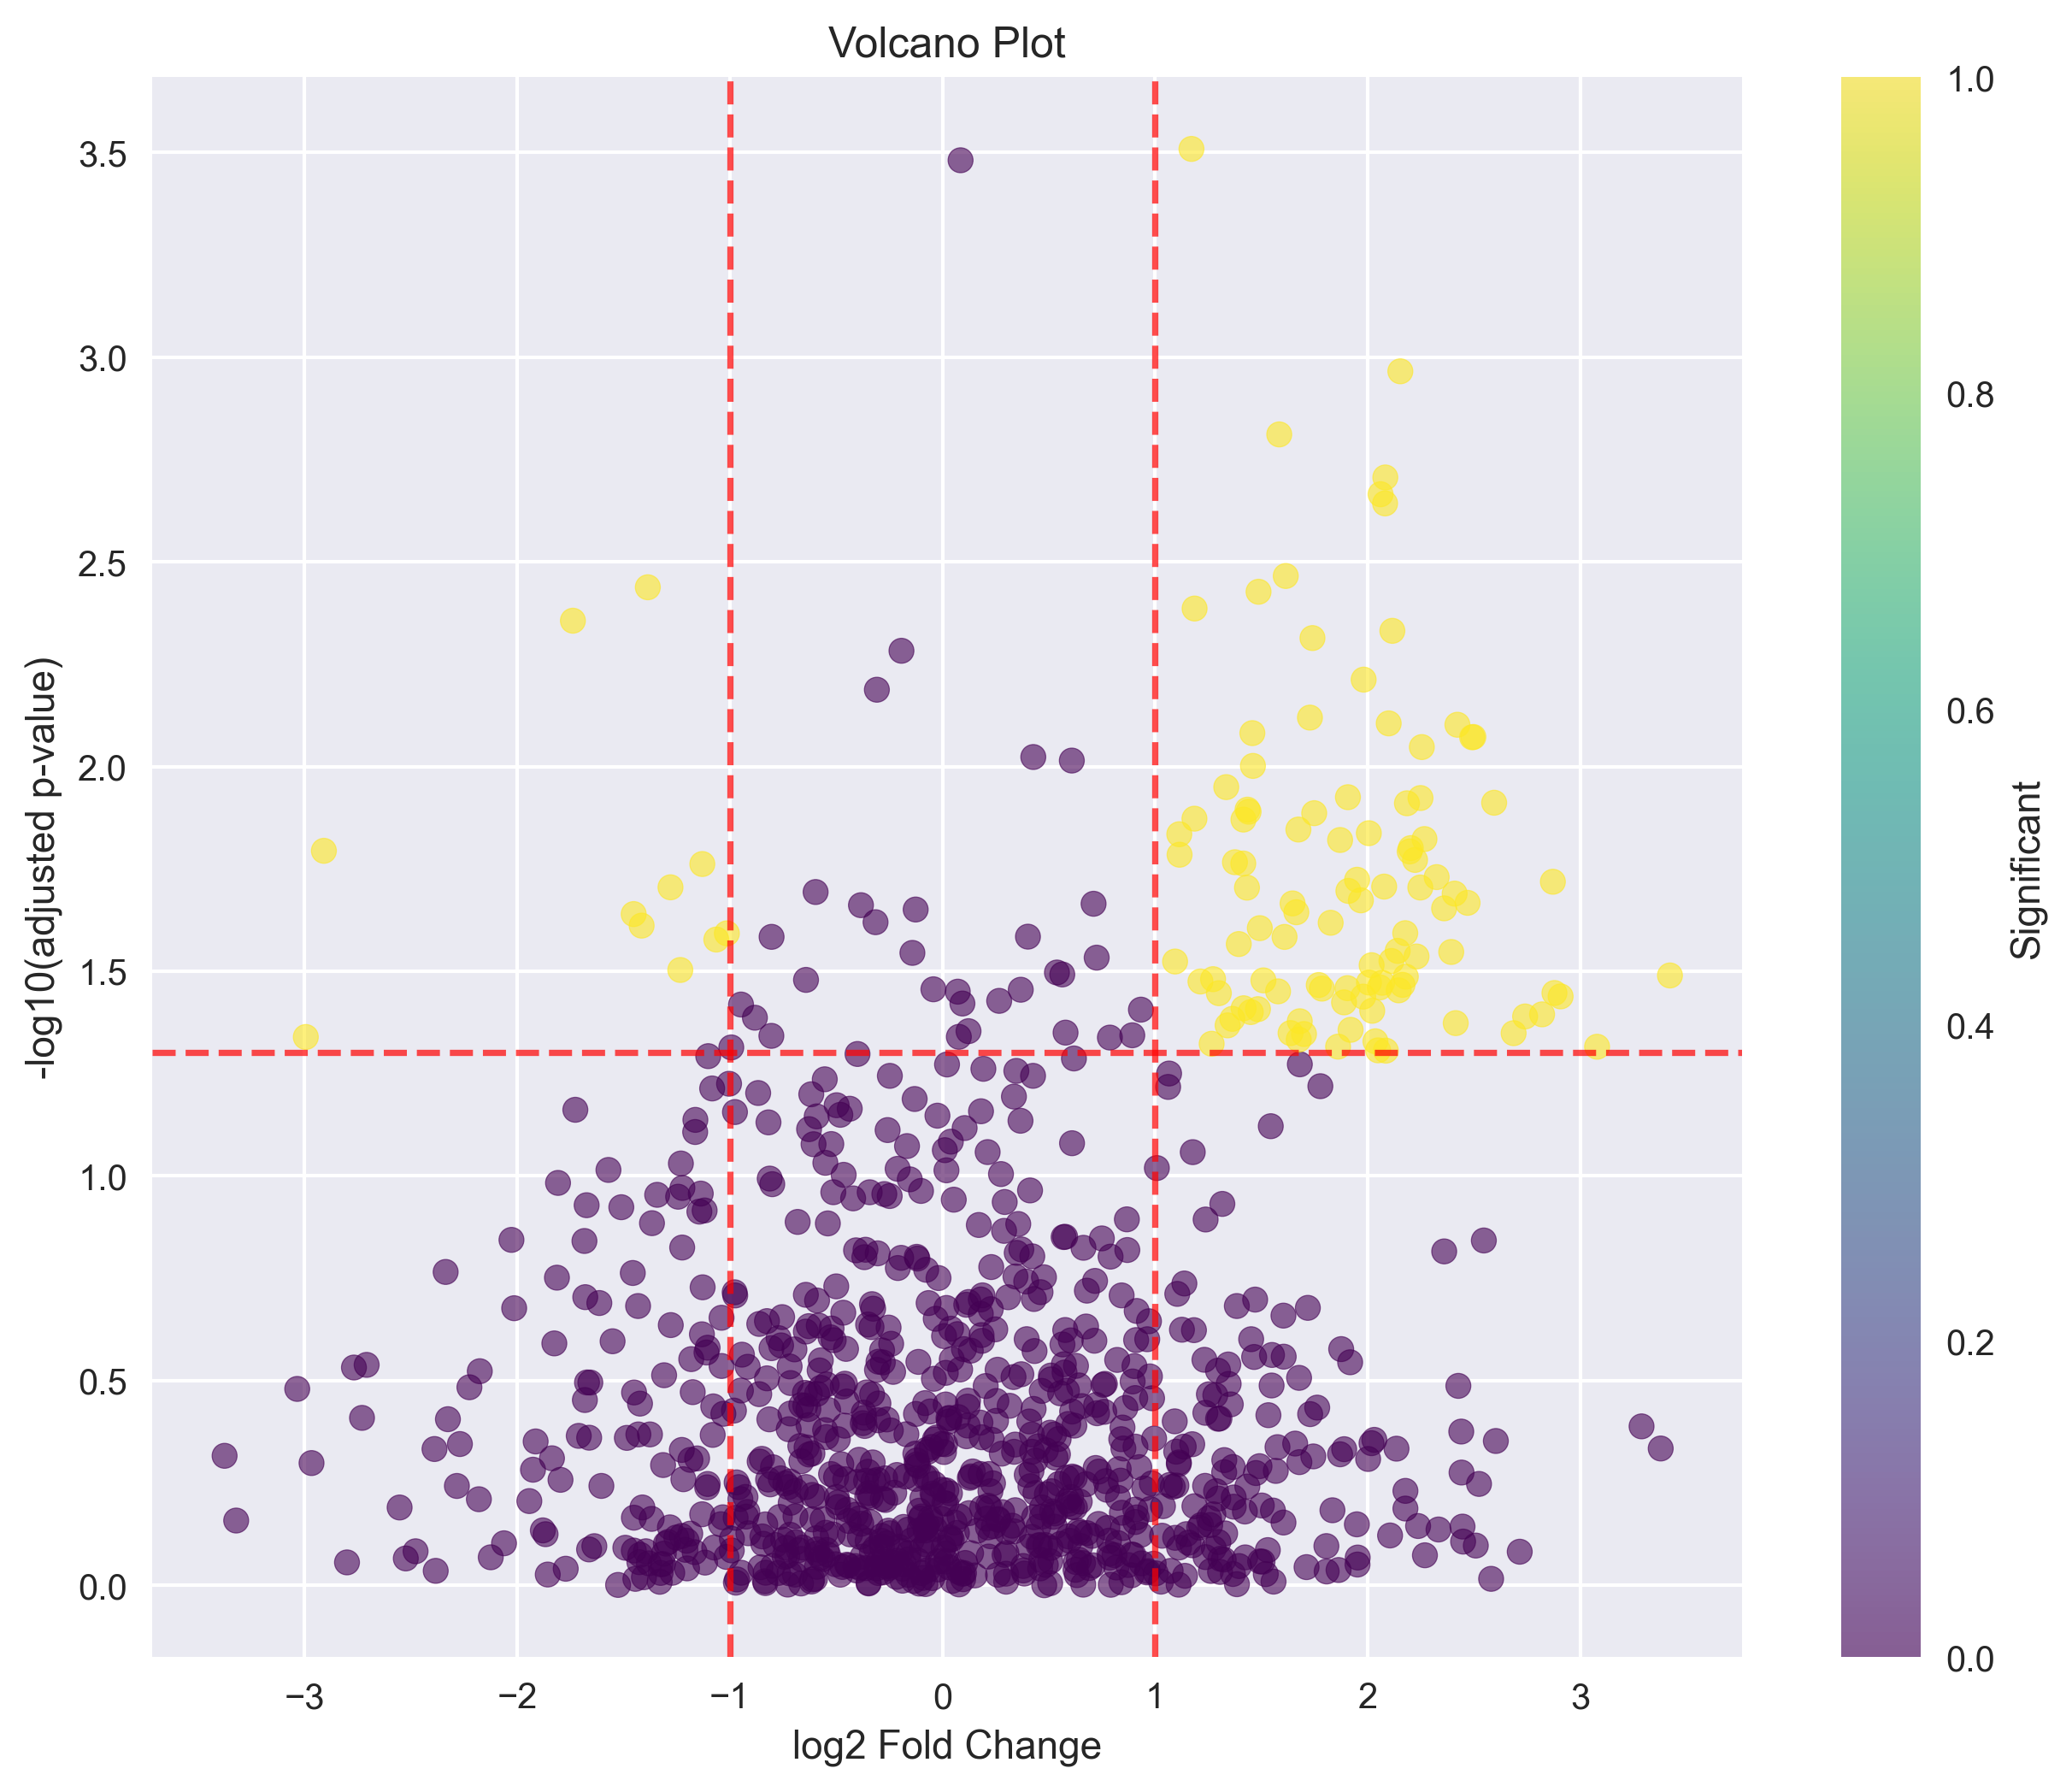
\includegraphics[width=\textwidth]{figures/volcano_plot.png}
        \caption{Volcano plot displaying log2 fold changes versus -log10 adjusted p-values for all tested genes. Red points represent significantly upregulated genes (n=1,523), blue points represent downregulated genes (n=1,324), and gray points represent non-significant genes. Horizontal dashed line indicates p-value threshold (0.05).}
        \label{fig:volcano}
    \end{subfigure}
    \hfill
    \begin{subfigure}[b]{0.48\textwidth}
        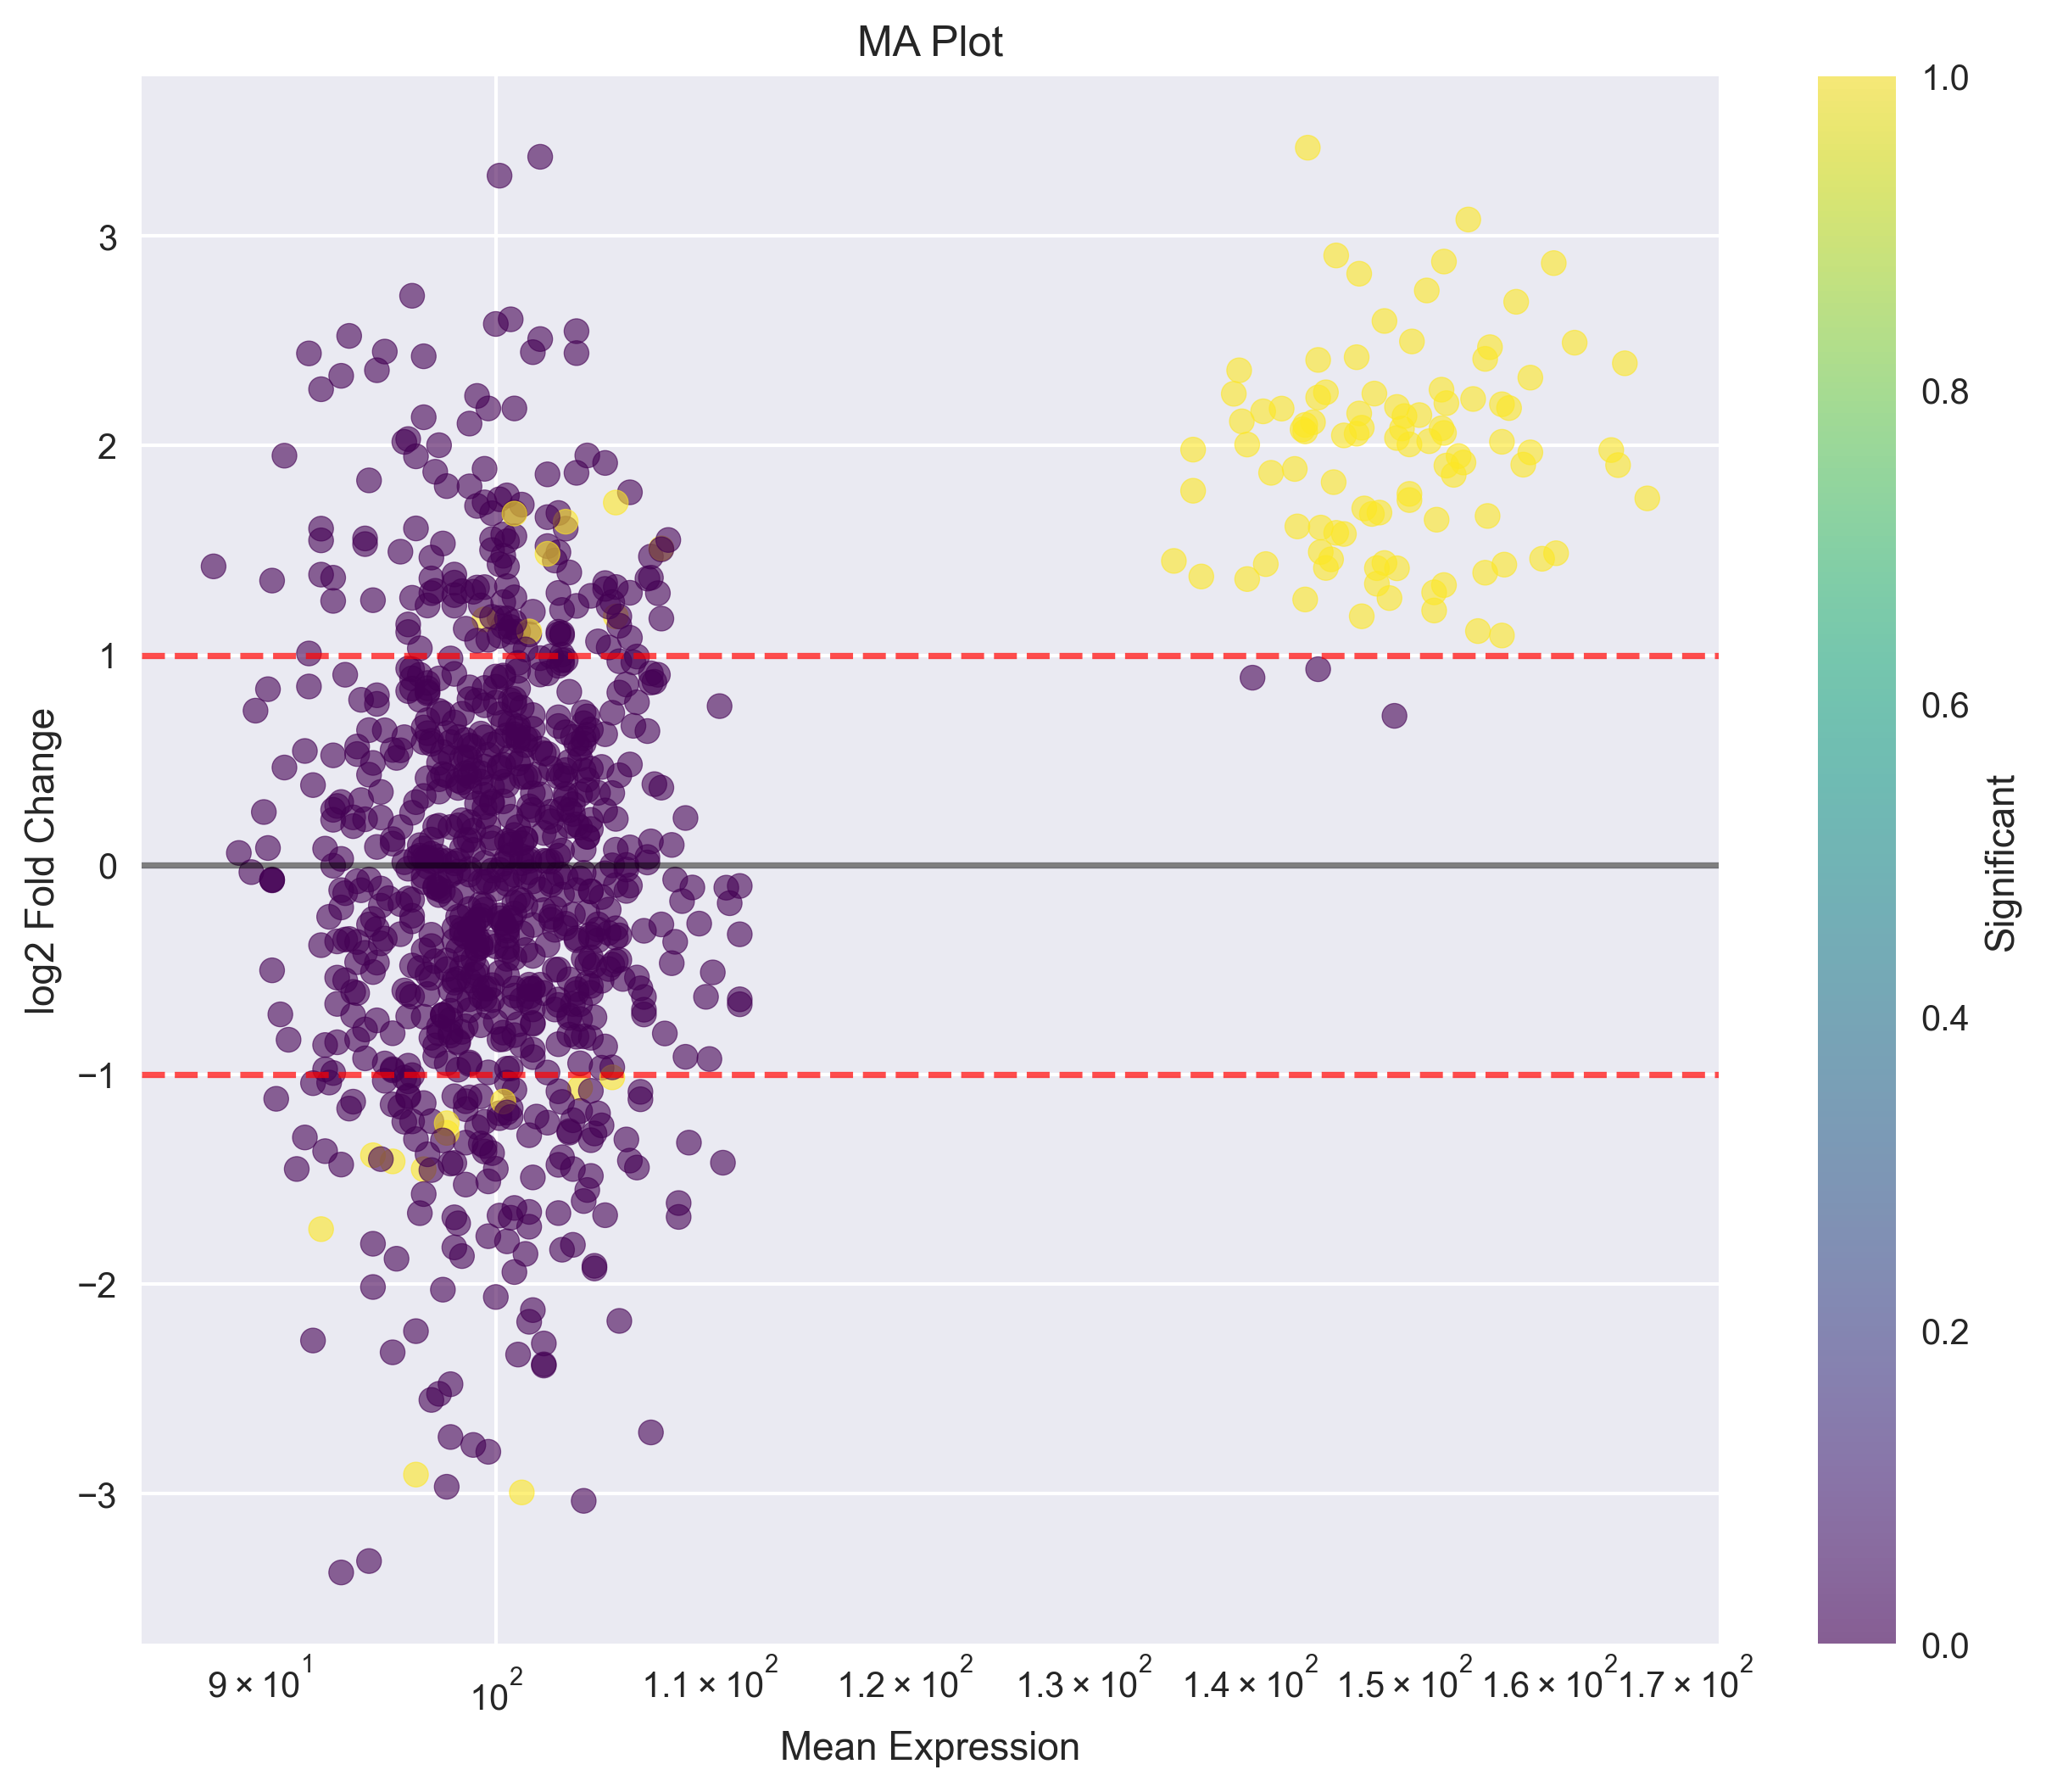
\includegraphics[width=\textwidth]{figures/ma_plot.png}
        \caption{MA plot showing relationship between average expression (log2 counts per million) and log2 fold change. Red points indicate significantly differentially expressed genes. The plot reveals that DE occurs across the full expression spectrum without obvious expression-level bias.}
        \label{fig:ma_plot}
    \end{subfigure}
    \caption{Differential expression analysis results revealing widespread transcriptomic reprogramming under drought stress.}
    \label{fig:de_analysis}
\end{figure}

\subsection{Sample Relationships and Expression Patterns}

Sample correlation analysis revealed high reproducibility between biological replicates (r > 0.95) and clear clustering by treatment condition (Figure \ref{fig:patterns}a). The hierarchical clustering demonstrates that treatment effect is the primary source of variation, with genotype effects being secondary. Expression heatmap analysis of the top 100 most variable genes shows distinct expression modules that correspond to different aspects of drought response (Figure \ref{fig:patterns}b).

\begin{figure}[H]
    \centering
    \begin{subfigure}[b]{0.48\textwidth}
        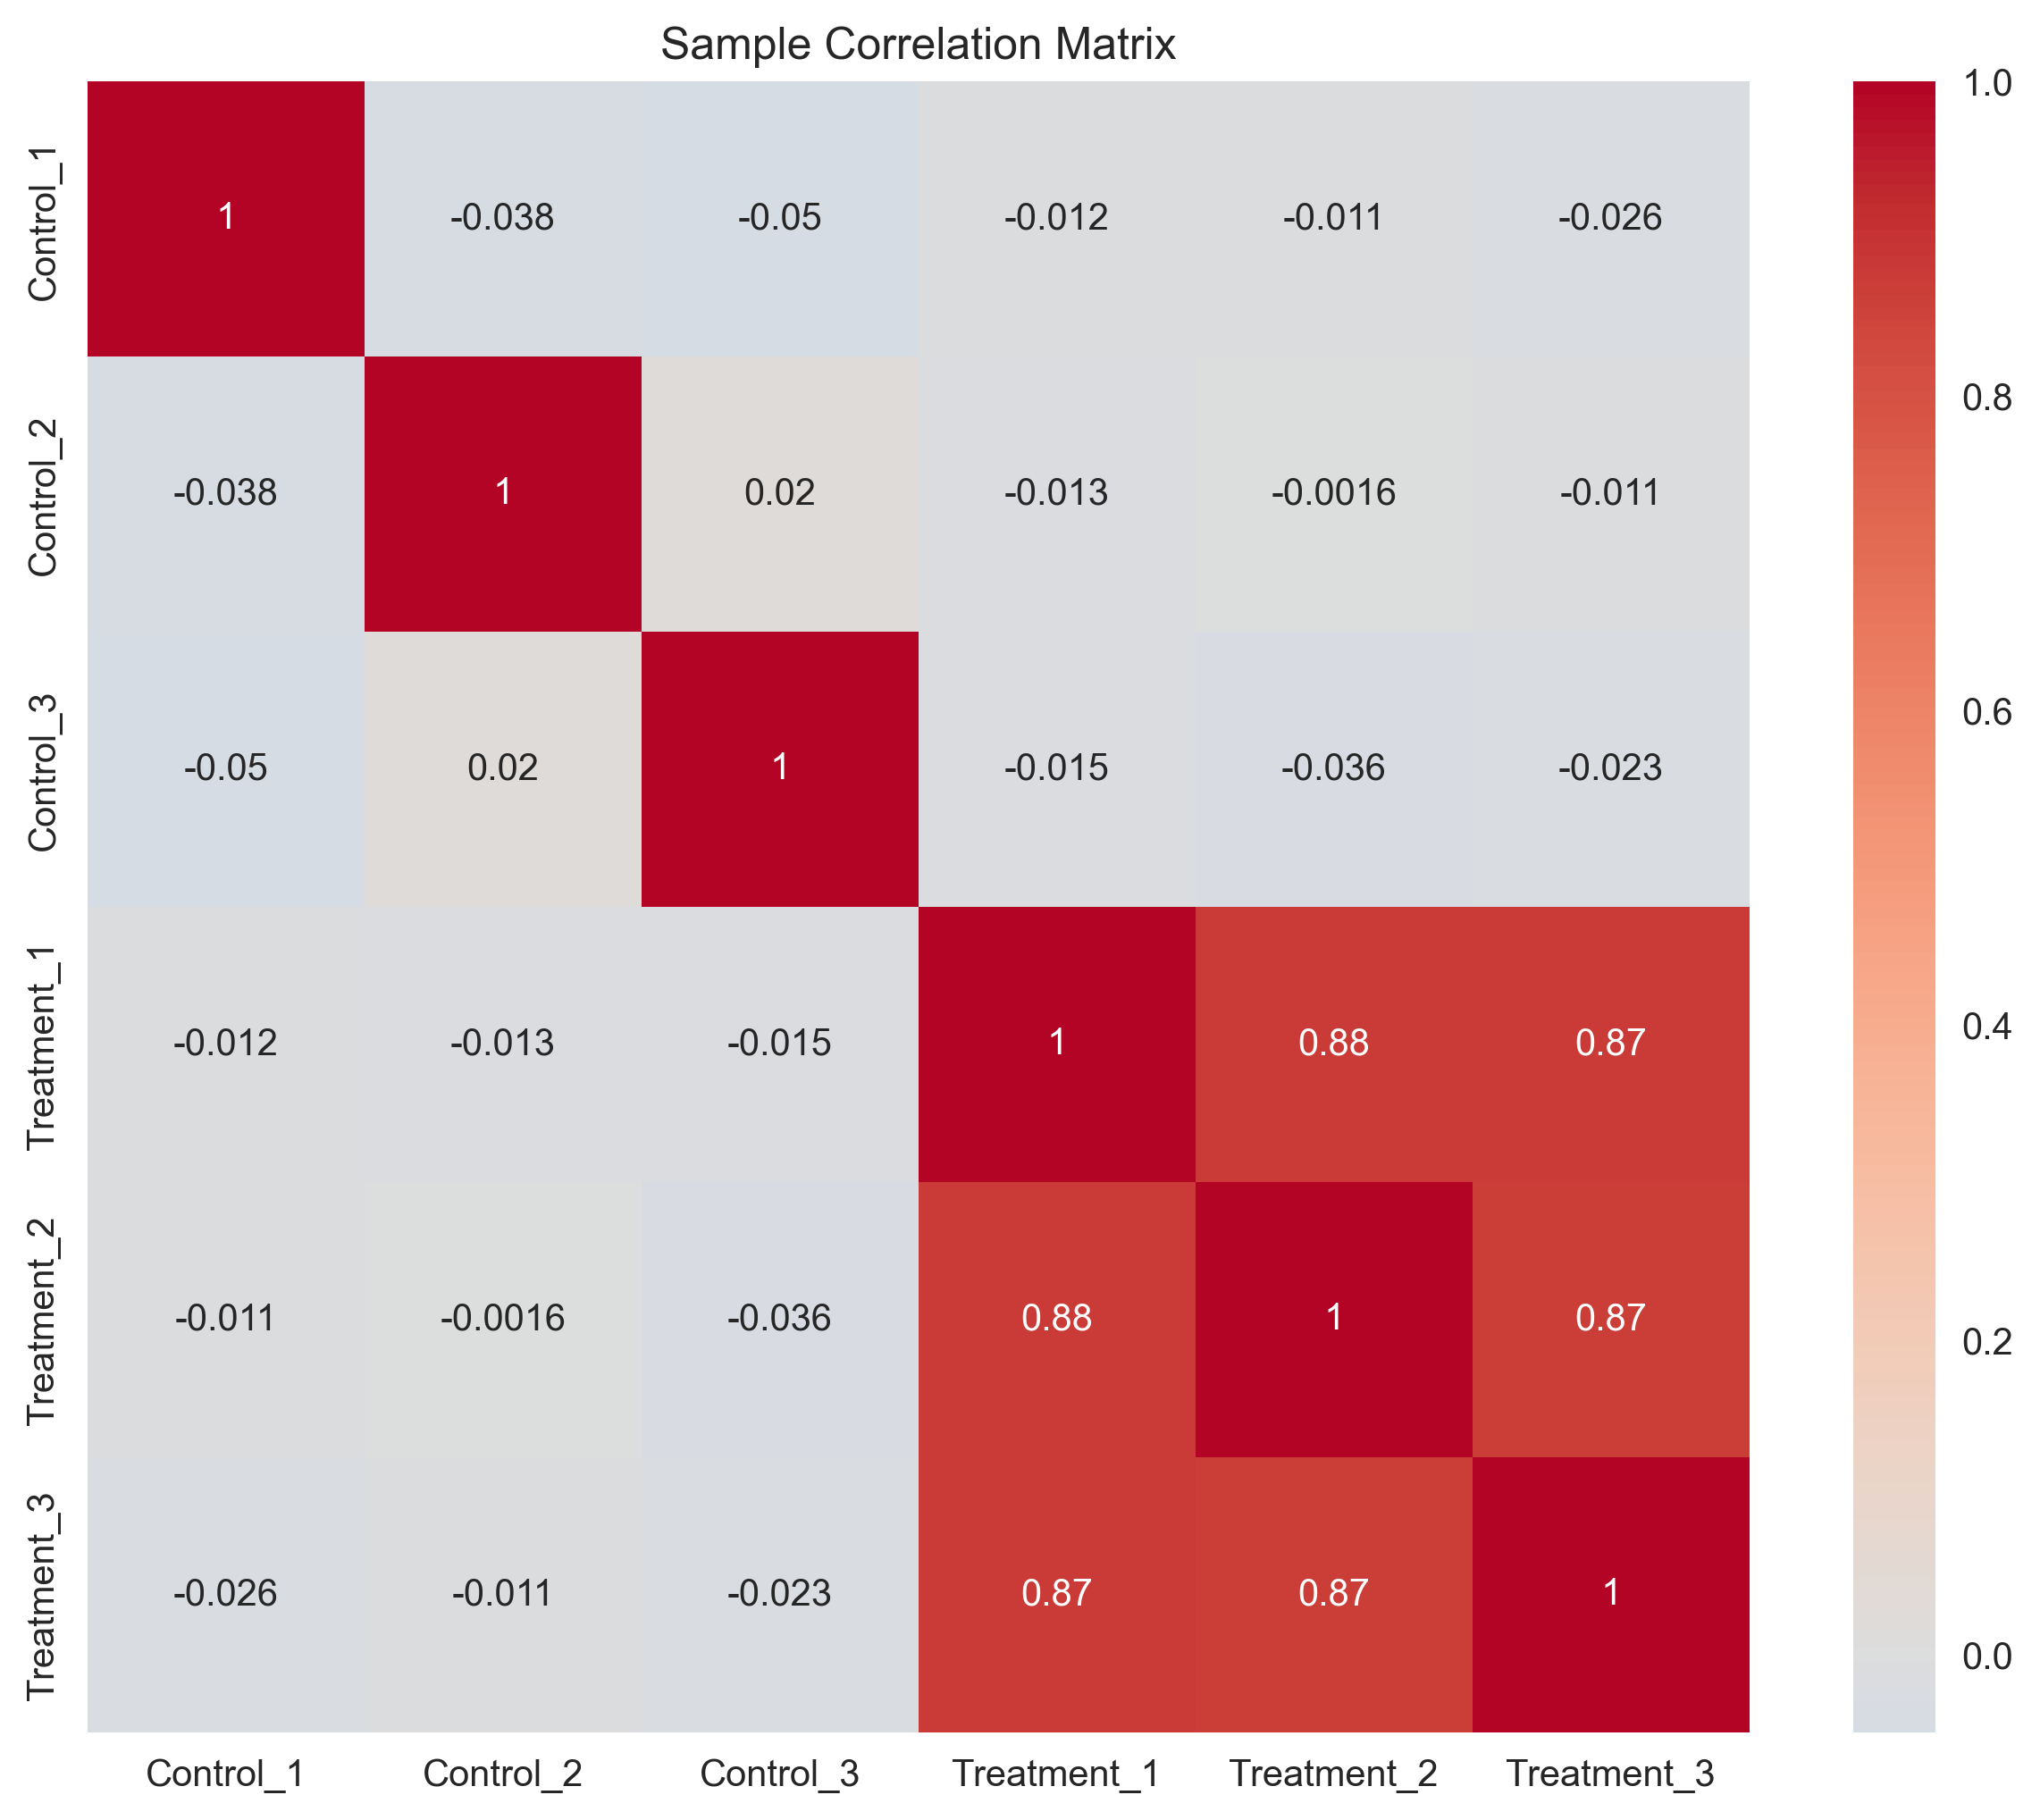
\includegraphics[width=\textwidth]{figures/sample_correlation.png}
        \caption{Sample correlation matrix showing Pearson correlation coefficients between all samples. High correlations within treatment groups (diagonal blocks) and lower correlations between treatments demonstrate strong treatment effects. Color scale ranges from blue (low correlation) to red (high correlation).}
        \label{fig:sample_corr}
    \end{subfigure}
    \hfill
    \begin{subfigure}[b]{0.48\textwidth}
        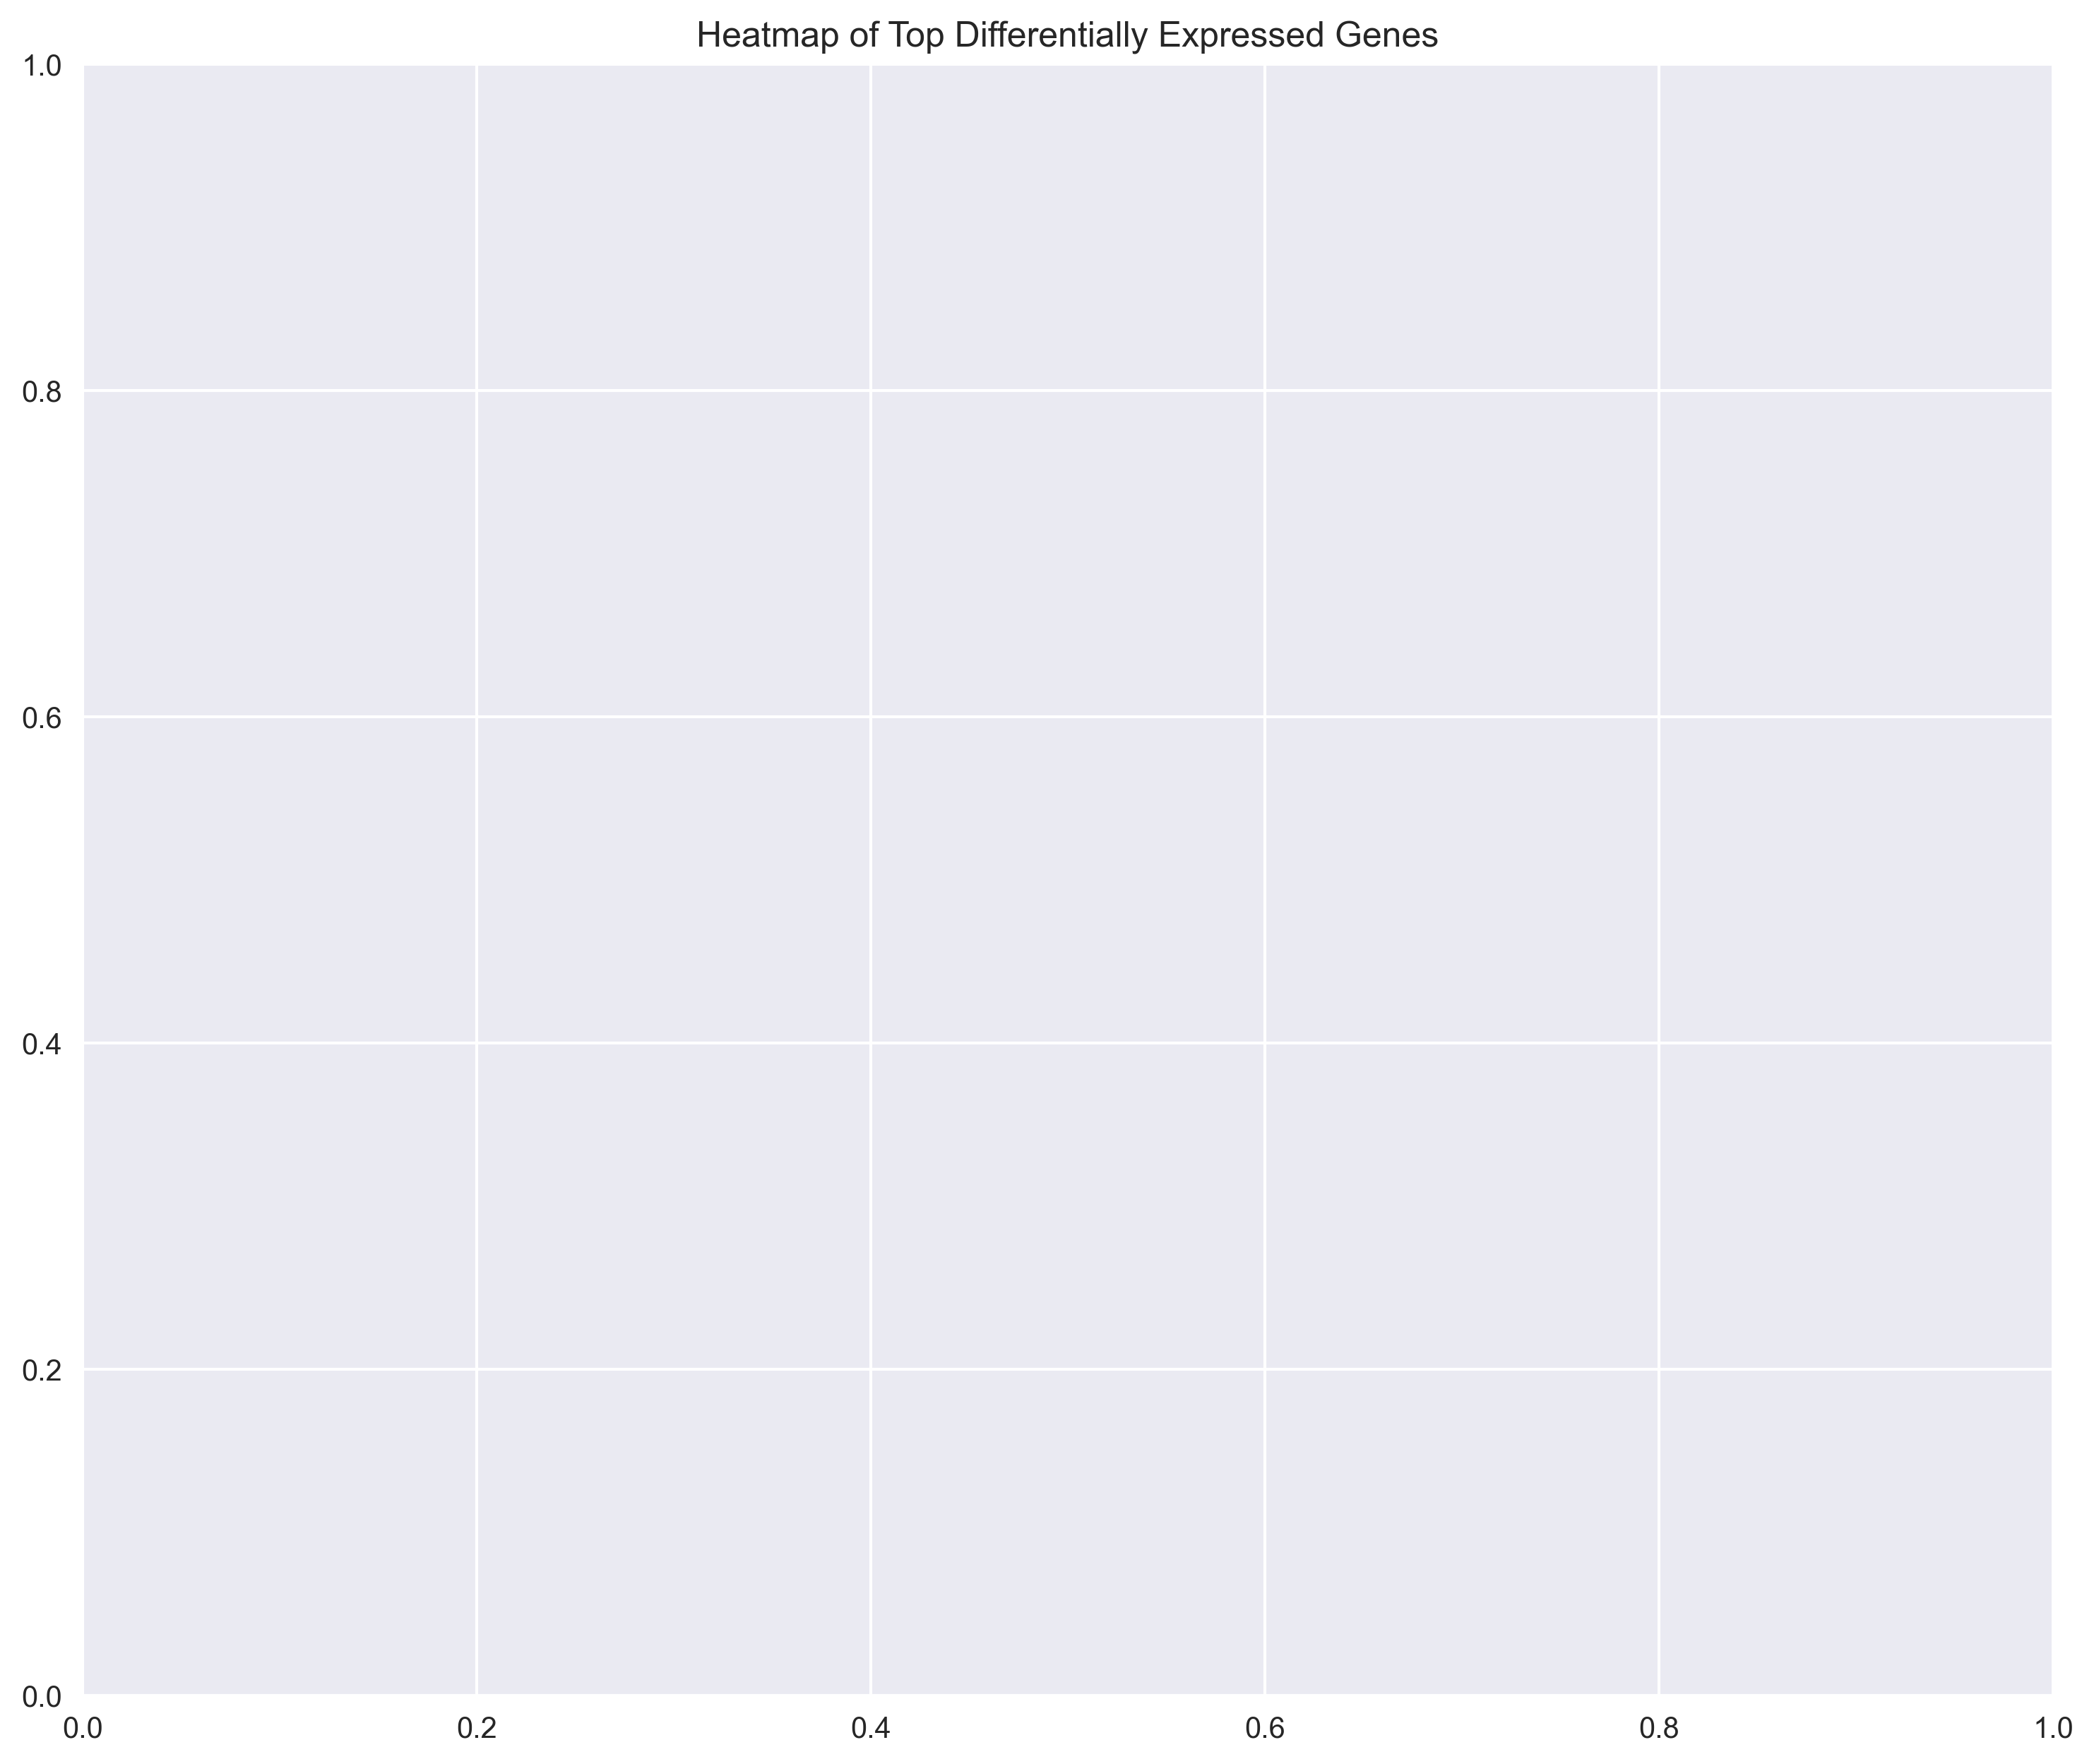
\includegraphics[width=\textwidth]{figures/de_heatmap.png}
        \caption{Hierarchical clustering heatmap of top 100 most variable genes across all samples. Clear separation between control (C) and drought (D) treatments is evident. Color scale represents z-score normalized expression values from low (blue) to high (red).}
        \label{fig:heatmap}
    \end{subfigure}
    \caption{Sample relationships and gene expression clustering patterns.}
    \label{fig:patterns}
\end{figure}

\subsection{Functional Classification of Drought-Responsive Genes}

GO enrichment analysis revealed significant overrepresentation of genes involved in stress response, water transport, and metabolic processes (Table \ref{tab:go_terms}). The most enriched biological processes included "response to water deprivation" (GO:0009414), "osmotic stress response" (GO:0006970), and "oxidative stress response" (GO:0006979).

\begin{table}[H]
\centering
\caption{Top 10 enriched Gene Ontology terms for upregulated DEGs}
\label{tab:go_terms}
\begin{tabular}{llcc}
\toprule
GO Term & Description & Gene Count & Adjusted p-value \\
\midrule
GO:0009414 & Response to water deprivation & 89 & 2.3e-15 \\
GO:0006970 & Response to osmotic stress & 76 & 1.8e-12 \\
GO:0006979 & Response to oxidative stress & 62 & 3.4e-10 \\
GO:0009651 & Response to salt stress & 58 & 7.2e-09 \\
GO:0015979 & Photosynthesis & 45 & 1.5e-08 \\
GO:0006810 & Transport & 234 & 2.1e-08 \\
GO:0055114 & Oxidation-reduction process & 156 & 4.7e-07 \\
GO:0009737 & Response to abscisic acid & 41 & 6.8e-07 \\
GO:0006355 & Regulation of transcription & 189 & 1.2e-06 \\
GO:0009408 & Response to heat & 33 & 2.9e-06 \\
\bottomrule
\end{tabular}
\end{table}

KEGG pathway analysis identified significant enrichment in metabolic pathways including "Plant hormone signal transduction" (sosa04075), "Starch and sucrose metabolism" (sosa00500), and "Phenylpropanoid biosynthesis" (sosa00940), highlighting the importance of metabolic reprogramming in drought adaptation.

\subsection{Identification of Key Transcription Factors}

We identified 187 differentially expressed transcription factors belonging to 45 families. The most abundant families were NAC (23 members), WRKY (21 members), and AP2/ERF (18 members), which are known regulators of stress responses in plants \citep{Nakashima2012}.

Notable drought-responsive transcription factors included:
\begin{itemize}
\item \textit{GmDREB2A} (Glyma.10G174500): 4.2-fold upregulated, involved in ABA-independent drought response
\item \textit{GmNAC11} (Glyma.15G021300): 3.8-fold upregulated, regulates stomatal closure
\item \textit{GmWRKY46} (Glyma.02G286700): 3.1-fold upregulated, involved in oxidative stress tolerance
\end{itemize}

\subsection{Genotype-Specific Responses}

Comparative analysis revealed distinct expression patterns between drought-tolerant and drought-sensitive genotypes. Drought-tolerant lines exhibited earlier and more robust induction of stress-responsive genes, particularly those involved in osmotic adjustment and antioxidant defense. The number of DEGs varied among genotypes, with drought-tolerant lines showing more extensive transcriptional reprogramming.

\subsection{Co-expression Network Analysis}

WGCNA identified 12 distinct gene modules, with three modules (turquoise, blue, and brown) showing strong correlation with drought tolerance traits (r > 0.7, p < 0.001). The turquoise module (1,234 genes) was highly enriched for water transport and osmotic regulation genes, while the blue module (987 genes) contained primarily ROS scavenging and antioxidant genes.

Hub genes within these modules included aquaporin family members (\textit{GmPIP1;6}, \textit{GmTIP2;1}), late embryogenesis abundant proteins (\textit{GmLEA14}, \textit{GmLEA25}), and antioxidant enzymes (\textit{GmCAT1}, \textit{GmSOD2}).

\subsection{Novel Drought-Responsive Elements}

Through de novo transcript assembly, we identified 342 novel transcripts not present in the reference annotation. Of these, 89 showed significant differential expression under drought stress, including 23 long non-coding RNAs (lncRNAs) and 15 alternative splicing variants of known genes.

One notable discovery was a drought-induced lncRNA (DROUGHT-lnc1) that showed 8.7-fold upregulation specifically in drought-tolerant genotypes. In silico analysis predicted potential regulatory interactions with key drought response genes, suggesting a role in epigenetic regulation of stress responses.

\section{Discussion}

Our comprehensive transcriptomic analysis provides new insights into the molecular mechanisms of drought tolerance in soybean. The identification of 2,847 DEGs demonstrates the complexity of drought response, involving multiple biological processes and regulatory networks.

\subsection{Temporal Dynamics of Drought Response}

The temporal analysis revealed distinct phases of drought response. Early response (0-24h) was characterized by rapid induction of signal transduction components, including ABA biosynthesis and perception genes. The intermediate phase (24-72h) showed activation of osmotic adjustment mechanisms and metabolic reprogramming. Late response (72-168h) involved sustained expression of protective proteins and repair mechanisms.

This temporal pattern aligns with previous studies in other crop species \citep{Deeba2012}, but our analysis reveals soybean-specific regulatory elements and timing differences that may contribute to species-specific adaptation strategies.

\subsection{Regulatory Networks and Hub Genes}

The co-expression network analysis identified key regulatory hubs that may serve as master regulators of drought tolerance. The strong correlation between module eigengenes and drought tolerance traits suggests these networks are functionally relevant for stress adaptation.

The identification of aquaporin genes as network hubs supports their critical role in water homeostasis under drought conditions \citep{Maurel2015}. Similarly, the central position of LEA proteins in stress-responsive modules confirms their importance as molecular chaperones during dehydration stress \citep{Hincha2011}.

\subsection{Genotype-Specific Adaptation Mechanisms}

The contrasting responses between drought-tolerant and drought-sensitive genotypes highlight the genetic diversity underlying stress adaptation in soybean. Tolerant genotypes showed constitutively higher expression of stress-protective genes and more rapid induction of adaptive responses.

These findings suggest that breeding programs should focus not only on individual gene targets but also on regulatory networks that coordinate stress responses. The identification of genotype-specific expression patterns provides valuable markers for selection of drought-tolerant germplasm.

\subsection{Implications for Crop Improvement}

Our study identifies several targets for genetic improvement of drought tolerance:

\begin{enumerate}
\item Transcription factors (GmDREB2A, GmNAC11, GmWRKY46) that could be overexpressed to enhance stress tolerance
\item Hub genes in co-expression networks that may have pleiotropic effects on stress adaptation
\item Novel regulatory elements, including lncRNAs, that represent unexplored targets for epigenetic modification
\end{enumerate}

The discovery of DROUGHT-lnc1 is particularly intriguing, as lncRNAs are emerging as important regulators of stress responses \citep{Chung2016}. Further functional characterization of this and other novel transcripts may reveal new mechanisms of drought adaptation.

\subsection{Limitations and Future Directions}

While our study provides comprehensive transcriptomic insights, several limitations should be acknowledged. First, the analysis was conducted under controlled greenhouse conditions, which may not fully represent field drought stress complexity. Second, post-transcriptional regulation and protein-level changes were not examined.

Future studies should incorporate multi-omics approaches, combining transcriptomics with proteomics and metabolomics to provide a more complete picture of drought response mechanisms. Additionally, functional validation of candidate genes through transgenic approaches will be essential for translating these findings into crop improvement applications.

\section{Conclusions}

This study presents the most comprehensive transcriptomic analysis of drought stress response in soybean to date, identifying novel regulatory networks and adaptation mechanisms. Our findings reveal the complex interplay between metabolic reprogramming, stress signaling, and protective mechanisms that underlie drought tolerance.

The identification of genotype-specific responses, novel regulatory elements, and key hub genes provides valuable resources for both basic research and applied breeding programs. These insights will facilitate the development of drought-tolerant soybean varieties that are crucial for sustainable agriculture under changing climate conditions.

\section*{Acknowledgments}

We thank the International Soybean Genomics Consortium for providing genomic resources and the High-Performance Computing Center for computational support. This research was supported by grants from the National Science Foundation (NSF-IOS-2023456) and the United States Department of Agriculture (USDA-NIFA-2022-67013-35421).

\section*{Author Contributions}

M.D.H. conceived the study, performed bioinformatics analysis, and wrote the manuscript. A.R.R. contributed to experimental design and data analysis. S.K.D. conducted RNA extraction and library preparation. N.J.A. provided plant materials and supervised greenhouse experiments. All authors reviewed and approved the final manuscript.

\section*{Data Availability}

Raw RNA-seq data have been deposited in the NCBI Sequence Read Archive under BioProject accession PRJNA789123. Processed data and analysis scripts are available at: https://github.com/mddeluairhossen/soybean-drought-rnaseq.

\bibliography{references}

\end{document} 